
\part{Préparer une Partie}

\section{Construire votre Liste d'Armée}
\label{building_an_army}

Batailles Fantastiques : Le 9\ieme{} Âge propose une série de Livres d'Armée qui décrivent les spécificités de chaque armée. Chaque armée regroupe un ensemble unique de personnages, troupes et règles. Les unités sont réparties en différentes catégories qui peuvent être contraintes à représenter une fraction minimale ou maximale du coût de l'armée.

La première étape de la construction d'une armée est d'écrire un choix d'unités, leurs options et leurs Coûts en Points sur un document qu'on appelle \og Liste d'Armée \fg{}. La composition d'une liste est sujette à des règles et restrictions, que l'on décrit en détails dans la suite du chapitre.

\subsection{Coût en points}

Chaque unité, arme, amélioration, Objet Magique, etc. vaut un certain montant de points. Le Coût en Points d'une unité est la somme des Coûts en Points de chacune de ses figurines et des options. Le Coût en Points d'une armée est la somme des Coûts en Points de toutes ses unités.


\newpage
\section{Restrictions}

Une armée de Batailles Fantastiques : Le 9\ieme{} Âge doit suivre des règles simples de composition, détaillées dans cette section.

\subsection{Coût en Points de l'armée}

Avant de construire une Liste d'Armée, mettez-vous d'accord avec votre adversaire sur la taille de la bataille, ou Coût en Points de l'armée. Le Coût en Points de l'armée, combinant la valeur de toutes les unités, équipements et options, ne doit pas dépasser la limite en points décidée pour la partie. Elle peut cependant descendre jusqu'à 40 points en dessous de cette limite.

\subsection{Catégories d'unités}

Les unités sont regroupées en différentes Catégories. Le nombre de points que l'on peut dépenser dans chaque Catégorie diffère selon l'armée et est défini dans le Livre d'Armée correspondant. La ou les Catégories auxquelles appartient une unité sont indiquées par des icônes placés à côté du nom de l'unité.

\begin{minipage}[c]{0.17\textwidth}
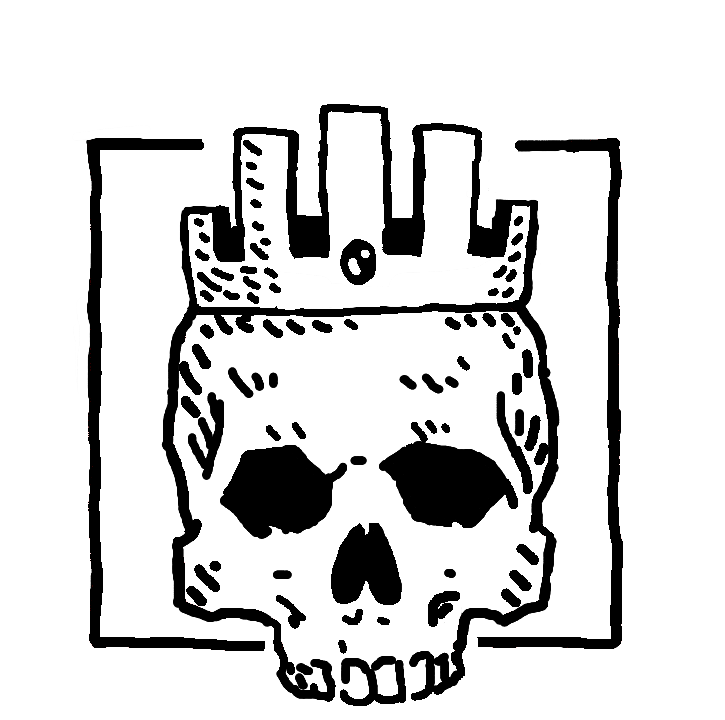
\includegraphics[width=\textwidth]{../Layout/pics/logo_lord.png}
\end{minipage}\hfill
\begin{minipage}[c]{0.80\textwidth}
\paragraph{Personnages}

Toute armée possède une Catégorie Personnage qui comprend des meneurs héroïques et de puissants \expandafter\lowercase\expandafter{\wizards}. Cette Catégorie est toujours limitée en terme de points que l'on peut y dépenser, habituellement 35\% du Coût en Points de l'armée. Toute unité appartenant à cette Catégorie est un Personnage et suit les règles correspondantes du chapitre \ref{characters} à la page \pageref{characters}.
\end{minipage}

\begin{minipage}[c]{0.17\textwidth}
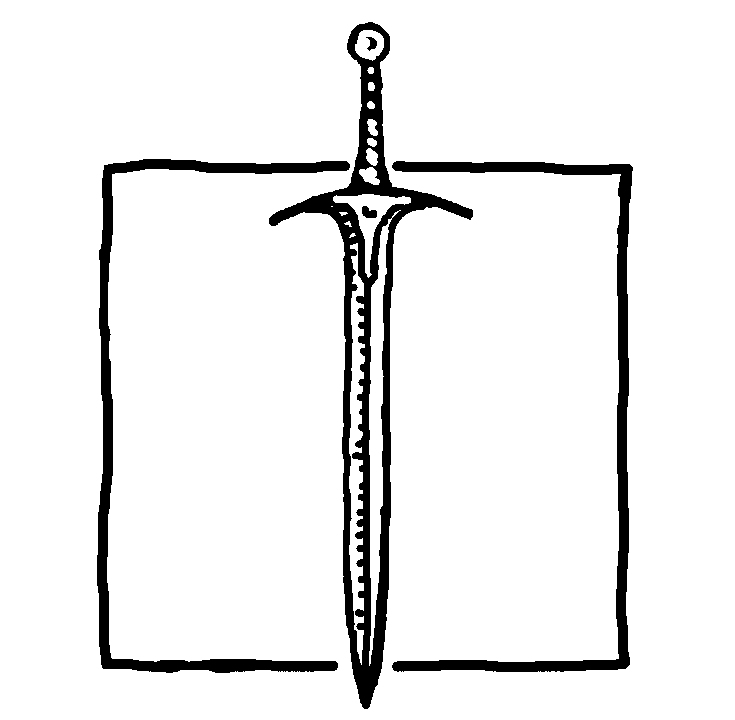
\includegraphics[width=\textwidth]{../Layout/pics/logo_core.png}
\end{minipage}\hfill
\begin{minipage}[c]{0.80\textwidth}
\paragraph{Unités de Base}

Les Unités de Base sont la colonne vertébrale d'une armée, toute armée doit en avoir. Cette catégorie a donc toujours une limite inférieure pour le nombre de points que l'on peut y dépenser, habituellement 25\% du Coût en Points de l'armée.
\end{minipage}

\begin{minipage}[c]{0.17\textwidth}
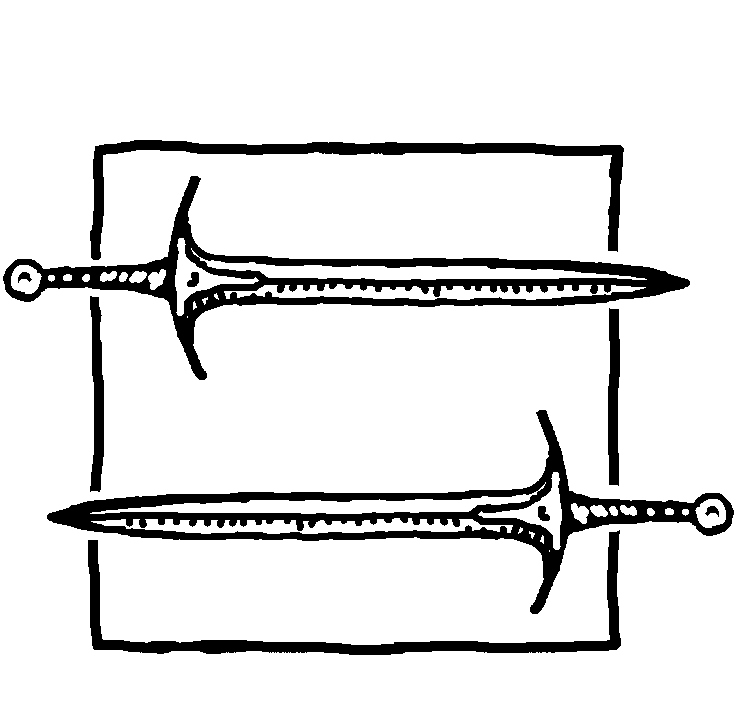
\includegraphics[width=\textwidth]{../Layout/pics/logo_special.png}
\end{minipage}\hfill
\begin{minipage}[c]{0.80\textwidth}
\paragraph{Unités Spéciales}

Cette catégorie n'a pas de limites, ni supérieure ni inférieure. Vous pouvez y dépenser autant de points que vous le souhaitez.
\end{minipage}

\begin{minipage}[c]{0.17\textwidth}

\includegraphics[width=\textwidth]{../Layout/pics/logo_specific.png}
\end{minipage}\hfill
\begin{minipage}[c]{0.80\textwidth}
\paragraph{Spécifique à l'Armée}

En plus des trois catégories génériques d'une armée que nous venons de présenter, toutes les armées possèdent au moins une Catégorie supplémentaire propre à elles dont les limites sont définies dans les Livres d'Armée.
\end{minipage}

\newpage
\paragraph{Unités appartenant à plus d'une Catégorie}

Certaines unités appartiennent à plusieurs Catégories. On les repère par la présence de plusieurs icônes à côté de leur nom dans le Livre d'Armée. Dans ce cas, le coût en point de l'unité doit simplement être comptabilisé pour les limites de toutes les Catégories dont elle fait partie. Il n'est cependant compté qu'une fois dans le Coût en Points de l'armée.

\paragraph{Ajouter des Catégories}

Certaines options peuvent faire compter une unité dans une nouvelle Catégorie en plus de leur Catégorie initiale. Par exemple, donner des armes de tir à une unité risque de la faire compter dans la Catégorie \og Soutien à Distance \fg{} de l'armée. Cela est indiqué par un petit icône de la Catégorie associée à l'option apparaissant à droite du nom de l'unité et par un texte descriptif accompagnant l'option.

\paragraph{Coût réparti dans plusieurs Catégories}

Dans quelques rares cas, le coût d'une unité peut être réparti dans différentes Catégories, par exemple quand une option compte dans une autre Catégorie que le reste de l'unité. Cela arrive pour les Montures de Personnages les plus effrayantes, comme les dragons. Le dragon peut par exemple compter dans la catégorie \og Bêtes et Monstres \fg{} tandis que son cavalier compte dans la Catégorie Personnages. Cela est indiqué par deux demi-icônes accolés, chaque moitié représentant une Catégorie : une pour l'unité et une pour l'option.

\subsection{Limites de duplication}

Certaines unités et options sont limitées en nombre. Il existe quatre types de restrictions.

\paragraph{0-X Unités par Armée}

Certaines unités ont la restriction \og 0-X Unités par Armée \fg{} (par exemple \og 0-2 Unités par Armée \fg{}). De telles unités peuvent être prises au plus en X exemplaires. La limite maximale (X) est divisée par 2 pour une Patrouille en arrondissant à l'unité supérieure, et multipliée par 2 pour une Grande Armée.

\paragraph{0-X Figurines par Armée}

Certaines unités ont la restriction \og 0-X Figurines par Armée \fg{} (par exemple \og 0-10 Figurines par Armée \fg{}). Cela signifie que, quelque soit le nombre d'exemplaires de l'unité inclus dans l'armée, le nombre total de leur figurines ne peut dépasser X. La limite maximale (X) est divisée par 2 pour une Patrouille en arrondissant à l'unité supérieure, et multipliée par 2 pour une Grande Armée.

\paragraph{0-X Choix par Armée}

Certaines améliorations ont la restriction \og 0-X Choix par Armée \fg{} (par exemple \og 0-2 Choix par Armée \fg{}). De telles améliorations peuvent être prises au plus en X exemplaires. La limite maximale (X) est divisée par 2 pour une Patrouille en arrondissant à l'unité supérieure, et multipliée par 2 pour une Grande Armée.

\paragraph{\oneperarmy}

Les unités, améliorations et objets avec la restriction \og \oneperarmy{} \fg{} ne peuvent être pris qu'en un seul exemplaire dans une armée. Cela ne change pas pour une Patrouille ou une Grande Armée.

\subsection{Restrictions additionnelles}

\paragraph{Taille d'Armée Minimale}

Une armée doit contenir au moins 4 unités sans compter les Personnages. On ne peut comptabiliser qu'une seule unité de type Machine de Guerre pour atteindre ce minimum.

\paragraph{Le Général}

Un des Personnages de l'armée doit être nommé Général. Il faut donc qu'il y ait au moins un Personnage dans l'armée capable de tenir ce rôle. Le Général doit être le Personnage ayant la plus grande valeur de Commandement de votre armée sans compter le Porteur de la Grande Bannière et les Personnages avec la règle \notaleader{}. Si plusieurs Personnages sont éligibles, vous pouvez choisir librement celui qui sera votre Général. Cela doit alors être précisé sur votre Liste d'Armée.

\section{Patrouilles et Grandes Armées}

Les règles de composition d'armée peuvent être modifiées selon la limite en points de la partie, si les armées sont plus petites ou grandes que la norme.

\begin{multicols}{2}\raggedcolumns

\begin{center}\textbf{Patrouilles}\end{center}

Les armées de 3000 points ou moins sont appelées Patrouilles. La taille d'armée minimale est réduite à 3 unités. La limite maximale (X) des restrictions 0-X Unités par Armée, 0-X Figurines par Armée et 0-X Choix par Armée est divisée par deux en arrondissant au supérieur.

\columnbreak

\begin{center}\textbf{Grandes Armées}\end{center}

Les armées de 8000 points ou plus sont appelées Grandes Armées. La limite maximale (X) des restrictions 0-X Unités par Armée, 0-X Figurines par Armée et 0-X Choix par Armée est doublée.

\end{multicols}

\newpage
\section{Liste d'Armée ouverte ?}

Les règles de ce jeu ont été équilibrées avec l'idée de listes d'armée complètement révélées. Par exemple, votre adversaire doit savoir quels Objets Magiques vos figurines possèdent. Nous encourageons les joueurs à partager leur Liste d'Armée complète avec leur adversaire au début de la partie, en détaillant unités, options, Objets Magiques, capacités spéciales, coûts en points, etc. Les seules choses qui ne doivent pas être montrées à votre adversaire sont celles explicitement citées comme cachées ou secrètes, comme par exemple dans quelle unité un Assassin est caché. Précisons que l'Assassin et son équipement sont quand même mentionnés dans la liste.

\subsection{Règles optionnelles pour listes cachées}
\label{hidden_lists}

Certains joueurs peuvent préférer jouer avec des listes dites \og cachées \fg{}. Rappelons que les règles du jeu n'ont pas été équilibrées dans cette optique. Dans ce cas, nous vous proposons de suivre les règles suivantes. La plus grande partie de votre armée doit rester connue de votre adversaire avant le début de la partie. Seuls quelques aspects sont secrets, ou \og cachés \fg{}. Les deux joueurs peuvent donner à leur adversaire une liste simplifiée dans laquelle les détails cachés sont omis.

Voilà les éléments qui peuvent être cachés : 

\begin{itemize}[label={-}]
\item Les Objets Magiques pris dans la liste commune de ce livre.
\item Les Objets Magiques spécifiques aux Livres d'Armée ainsi que toute option suivant les règles des Objets Magiques, comme les Objets Démoniaques et les Runes Naines.
\end{itemize}

Le reste doit être présenté dans la partie ouverte de votre liste. De plus, les Objets Magiques et assimilés qui ont un équivalent standard doivent être présentés sur la liste ouverte comme tels. Une Arme Lourde magique, par exemple, apparait comme une simple Arme Lourde.

Quand vous possédez au moins deux unités qui sont identiques dans la liste ouverte, mais qui ont une différence cachée, comme par exemple une Bannière Magique, vous devez avoir un moyen visible de les différencier, noté sur votre liste complète. Par exemple, la bannière rouge est la Bannière Magique, tandis que la bleue est ordinaire.

\paragraph{Révéler les Objets Magiques}

Un Objet Magique, ou équivalent, doit être révélé à la première utilisation. Un objet est considéré comme utilisé quand il a une chance d'affecter le jeu d'une quelconque façon. Entre autres :
\begin{itemize}[label={-}]
\item si cela affecte un jet de dé, même si le résultat obtenu sur le dé ne déclenche pas d'effet ;
\item si cela altère une attaque, via une Arme Magique ou tout objet dont une règle affecte l'attaque ;
\item si cela altère un jet de sauvegarde. L'objet doit alors être révélé avant que les dés ne soient jetés. Remarquez qu'un objet qui affecte une sauvegarde de la même manière que son équivalent standard le ferait, comme un Bouclier Magique, ne doit pas forcément être révélé.
\end{itemize}

Un objet qui augmente la mobilité ne compte comme étant utilisé que lorsque l'unité se déplace plus loin qu'elle ne le pourrait sans l'objet, ou lorsqu'elle charge. Déclarez alors l'objet avant de lancer le jet de distance de charge, mais après que les réactions ont été déclarées. Pour les Objets Runiques Nains, ne révélez que la Rune qui est utilisée, pas la combinaison complète.

